% ==========================================================
% Póster académico A1 horizontal · 3 columnas
% Proyecto Integrador · Maestría en Inteligencia Artificial Aplicada
% Basado en poster/template/poster_plantilla.tex (sin logo derecho).
% Contenido: artículo (producto_difusion) y resumen ejecutivo.
% Compilación: pdfLaTeX (Charter para títulos).
% ==========================================================
\documentclass[10pt]{article}

\usepackage{iftex}
\usepackage[a1paper,landscape,margin=1.5cm]{geometry}
\usepackage[spanish,es-noshorthands]{babel}
\usepackage{xcolor}
\usepackage{graphicx}
\usepackage{tikz}
\usetikzlibrary{arrows.meta,positioning}
\usepackage[most]{tcolorbox}
\usepackage{enumitem}
\usepackage{booktabs}
\usepackage{colortbl}
\usepackage{microtype}

% ---------------------- TIPOGRAFÍA -------------------------
\ifTUTeX
  \usepackage{fontspec}
  \IfFontExistsTF{Instrument Serif}%
    {\newfontfamily\serif{Instrument Serif}}%
    {\newfontfamily\serif{TeX Gyre Pagella}}
\else
  \usepackage[utf8]{inputenc}
  \usepackage[T1]{fontenc}
  \usepackage{lmodern}
  \usepackage[scaled=0.95]{helvet}
  \newcommand{\serif}{\fontfamily{bch}\selectfont}
\fi

\pagestyle{empty}
\setlength{\parindent}{0pt}
\setlength{\parskip}{0.4em}

% ---------------------- PALETA -----------------------------
\definecolor{olive}{HTML}{9AA542}
\definecolor{olivedark}{HTML}{1B2208}
\definecolor{olivelink}{HTML}{6B7A1F}
\definecolor{olivesoft}{HTML}{E4E8C7}
\definecolor{ink}{HTML}{1A1A10}
\definecolor{muted}{HTML}{6B6B5E}
\definecolor{pagebg}{HTML}{FFFFFF}

\pagecolor{pagebg}
\color{ink}

% ---------------------- DATOS DEL PÓSTER -------------------
\newcommand{\programa}{Maestría en Inteligencia Artificial Aplicada}
\newcommand{\tituloA}{Parada anticipada del MSAPSO}
\newcommand{\tituloB}{para el seguimiento del punto de máxima potencia bajo sombra parcial}
\newcommand{\autores}{P.\,C. Márquez Correo\quad D. Molina León\quad F. Moreira Guerra}
\newcommand{\asesor}{Prof. Gerardo J. Camacho González, PhD}
\newcommand{\fecha}{Noviembre 2026}

\newcommand{\logoizq}{
\includegraphics[height=5cm]{template/logo.jpeg}}

% ---------------------- ESTILOS ----------------------------
\newcommand{\seccion}[1]{%
  \begin{tcolorbox}[colback=olive,colframe=olive,arc=0pt,
    boxrule=0pt,left=8pt,top=3pt,bottom=4pt,width=\linewidth]
    {\serif\color{white}\fontsize{30}{36}\selectfont #1}
  \end{tcolorbox}\vspace{-0.3em}}

\newcommand{\cuerpo}{\fontsize{24}{31}\selectfont}

\newcommand{\circulo}[1]{%
  \tikz\node[circle,fill=olivesoft,minimum size=5.2cm,align=center,
    text width=4.6cm,text=olivedark,
    font=\sffamily\bfseries\fontsize{19}{23}\selectfont]{#1};}

\newcommand{\pie}[1]{{\sffamily\fontsize{18}{22}\selectfont\color{muted}#1}}

\newlength{\hdrh}\setlength{\hdrh}{9cm}
\newlength{\colh}
\setlength{\colh}{\dimexpr\textheight-\hdrh-6cm\relax}

% ======================================================
\begin{document}

% ---------------------- ENCABEZADO ------------------------
% Sin logo derecho: la columna derecha queda vacía para mantener el título centrado.
\noindent\parbox[t][\hdrh][c]{\linewidth}{%
\begin{minipage}[c]{0.21\linewidth}
  \raggedright\logoizq
\end{minipage}%
\begin{minipage}[c]{0.62\linewidth}
  \centering
  {\serif\fontsize{58}{65}\selectfont\color{olivedark}\tituloA\par}
  {\serif\fontsize{38}{46}\selectfont\color{olivedark}\tituloB\par}
  \vspace{0.5em}
  {\sffamily\bfseries\fontsize{30}{36}\selectfont\color{olivelink}\programa\par}
  \vspace{0.3em}
  {\fontsize{26}{32}\selectfont\color{ink}\autores\par}
  {\fontsize{22}{28}\selectfont\color{muted}Asesor: \asesor\ \textperiodcentered\ \fecha\par}
\end{minipage}%
\begin{minipage}[c]{0.17\linewidth}
  \hfill
\end{minipage}}

\vspace{0.4cm}
{\color{olive}\rule{\linewidth}{2.5pt}}
\vspace{0.6cm}

% ---------------------- COLUMNAS --------------------------
\noindent
\begin{minipage}[t][\colh][s]{0.30\linewidth}\cuerpo\vspace{0pt}
% ===== COLUMNA IZQUIERDA =====

\seccion{Contexto de negocio y problema}
Un panel fotovoltaico entrega su máxima potencia en un solo punto de operación. Con \textbf{sombra parcial} la curva potencia--corriente tiene varios máximos, y el controlador debe buscar el mayor midiendo en distintas corrientes; mientras busca, el panel entrega menos de lo que podría.

El referente es el \textbf{MSAPSO}, un enjambre determinista de 7 partículas: es preciso, pero con sombra cambiante busca una y otra vez. Proyecto exploratorio, sin fin comercial. \textbf{Pregunta:} ¿hay un método que supere al MSAPSO en energía con menos mediciones, sin empeorar su exactitud ni su cola de riesgo?

\begin{center}
  \begin{tikzpicture}
    \fill[olivesoft] (0,0) arc (180:0:3.6 and 3.6) -- (4.8,0) arc (0:180:2.4 and 2.4) -- cycle;
    \node[font=\serif\fontsize{56}{60}\selectfont,text=olivedark] at (3.6,0.9) {175};
  \end{tikzpicture}\\[2pt]
  \pie{Mediciones por búsqueda del MSAPSO, siempre.}
\end{center}

\vfill
\seccion{Datos y preparación}
\begin{itemize}[leftmargin=1.2em,itemsep=0.5em]
  \item \textbf{Fuentes:} los cuatro casos del manuscrito base y un generador de sombras sintéticas. Todo es simulación.
  \item \textbf{Simulador dinámico:} convertidor Boost (10~mH, carga de 12~$\Omega$) con control Super-Twisting; la eficiencia se mide contra el máximo \textit{alcanzable}.
  \item \textbf{2\,400 escenarios} con semillas fijas: ajuste (600--1199), prueba (0--599) y confirmación (1200--2399), nunca usada para decidir.
\end{itemize}

\vfill
\seccion{Metodología y modelos}
\begin{itemize}[leftmargin=1.2em,itemsep=0.5em]
  \item \textbf{Protocolo único:} energía entregada, IC 95\,\% (\textit{bootstrap} pareado) y criterios previos: ventaja demostrable y cola p99 $\le$ 3~pp.
  \item \textbf{11 métodos:} redes neuronales (MLP + CEM), entropía cruzada (CEM, DecentCEM) y poblacionales (DGBCO, CEDGO), con sus variantes.
  \item \textbf{Modelo final, V7:} el mismo MSAPSO, pero se detiene cuando las partículas se agrupan (dispersión $<$ 2\,\% de $I_{sc}$, mínimo 3 pasadas). Sin entrenamiento.
\end{itemize}

\end{minipage}\hfill
\begin{minipage}[t][\colh][s]{0.37\linewidth}\cuerpo\vspace{0pt}
% ===== COLUMNA CENTRAL =====

\begin{center}
  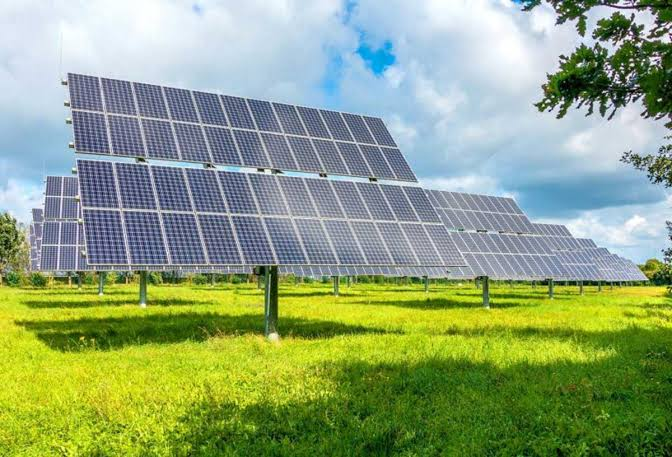
\includegraphics[width=\linewidth,height=10.5cm,keepaspectratio]{imagenes/paneles_solares.jpg}\\[2pt]
  \pie{Figura 1. Arreglo fotovoltaico (imagen ilustrativa).}
\end{center}

\vfill
\seccion{Resultados y validación}

En 1\,200 escenarios de confirmación la \textbf{V7 entrega 87.38\,\%} de la energía máxima contra 84.60\,\% del MSAPSO: \textbf{+2.78~pp} [IC 95\,\%: 2.39, 3.18], con \textbf{70 mediciones en lugar de 175} y solo 0.05~pp menos de exactitud. La ventaja se concentra donde la sombra cambia con frecuencia (+6.7~pp en régimen alto) y no hay sobreajuste (+3.58, +2.98 y +2.78~pp en ajuste, prueba y confirmación).

\begin{center}
  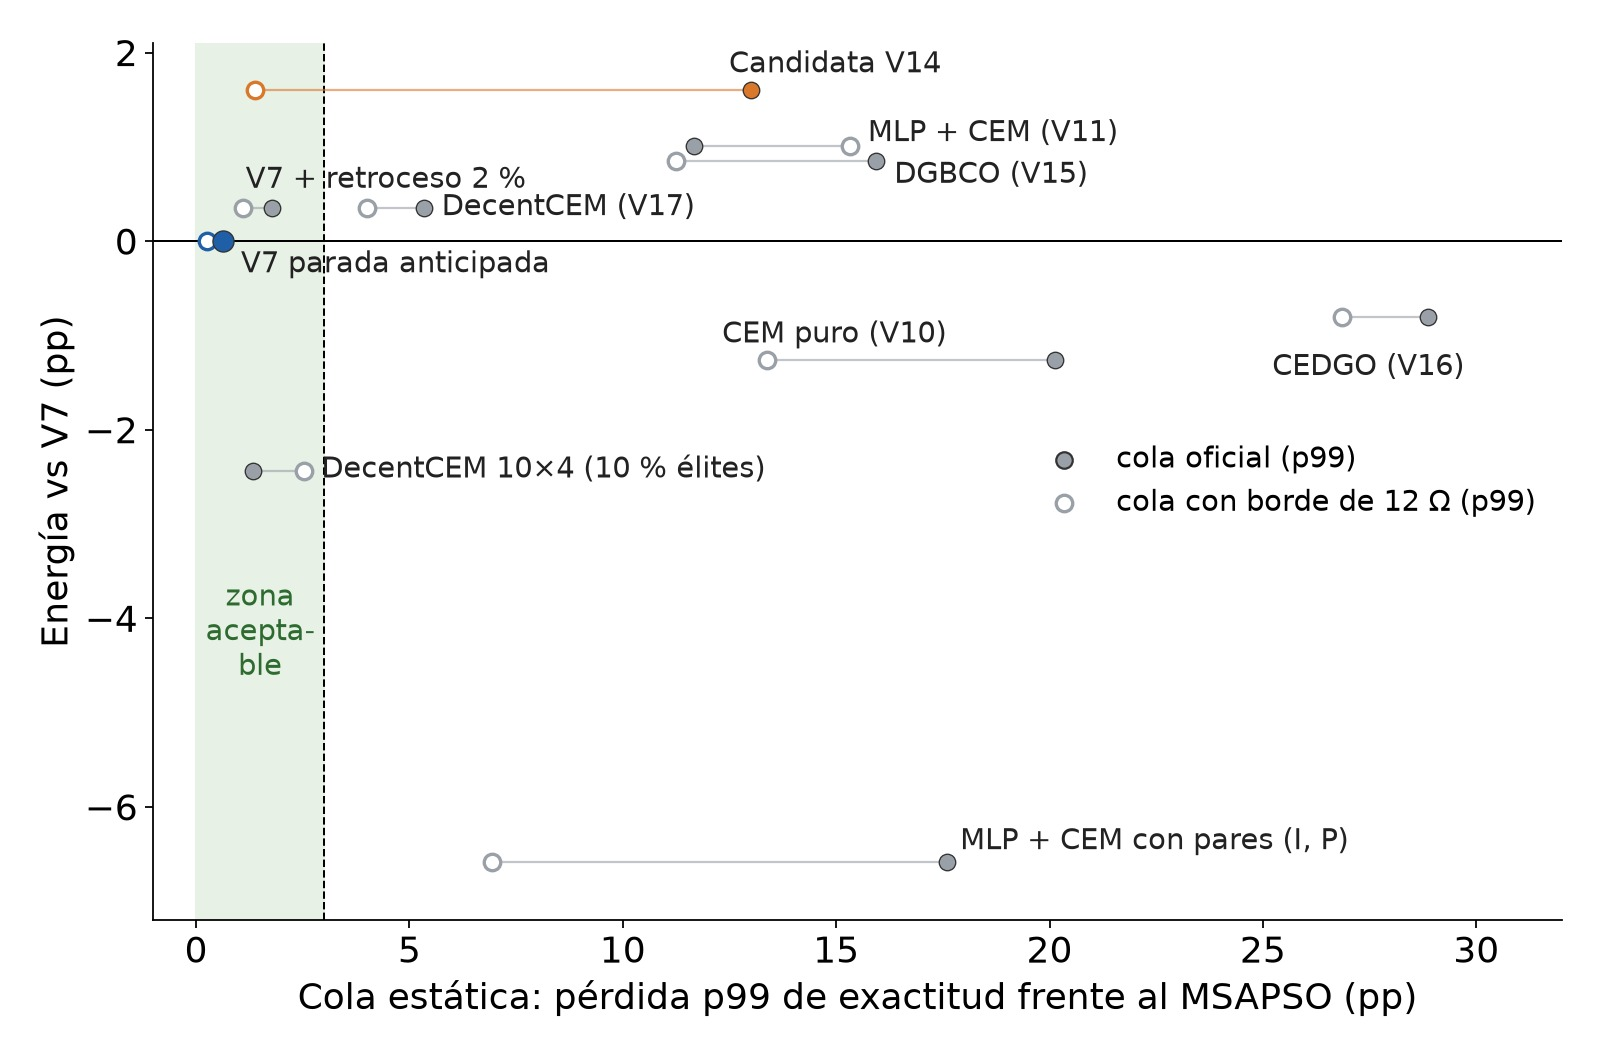
\includegraphics[width=0.95\linewidth,height=11.5cm,keepaspectratio]{imagenes/fig3_energia_cola.jpg}\\[2pt]
  \pie{Figura 2. Energía frente a la V7 contra cola p99 (lleno: oficial; hueco: con límite de 12~$\Omega$).}
\end{center}

\vfill
\seccion{Arquitectura de despliegue}
\begin{center}
\begin{tikzpicture}[
  paso/.style={rectangle,rounded corners=10pt,fill=olivesoft,align=center,
    font=\sffamily\fontsize{20}{25}\selectfont,text=olivedark,
    text width=7.2cm,minimum height=5.2cm,inner sep=10pt},
  arr/.style={-{Stealth[length=6mm]},line width=4pt,color=olive}]
  \node[paso] (a) at (0,0)
    {\textbf{Validación}\\[4pt]Simulador y banco \textit{hardware-in-the-loop}};
  \node[paso] (b) at (9.4,0)
    {\textbf{Controlador (borde)}\\[4pt]Búsqueda V7 en firmware, $\approx$ 30 operaciones por pasada};
  \node[paso] (c) at (18.8,0)
    {\textbf{Nube}\\[4pt]Telemetría, alertas y versiones firmadas};
  \draw[arr] (a.east) -- (b.west);
  \draw[arr] (b.east) -- (c.west);
\end{tikzpicture}
\end{center}

\end{minipage}\hfill
\begin{minipage}[t][\colh][s]{0.30\linewidth}\cuerpo\vspace{0pt}
% ===== COLUMNA DERECHA =====

\seccion{Conclusiones clave}
La mejora que sobrevivió a todas las pruebas fue la más simple: \textbf{detener el enjambre cuando se agrupa}. Ningún método gana energía a la V7 y cumple a la vez la cola.

\begin{center}
\pie{Tabla 1. Métodos en la confirmación. Cola p99 en pp; entre paréntesis, con límite de 12~$\Omega$.}

\vspace{0.3em}
\fontsize{20}{25}\selectfont
\renewcommand{\arraystretch}{1.12}
\arrayrulecolor{olivedark}
\begin{tabular}{lrrr}
  \toprule
  \textbf{Método} & \textbf{Med.} & \textbf{vs V7 (pp)} & \textbf{Cola p99} \\
  \midrule
  MSAPSO & 175 & $-2.78$ & --- \\
  \textbf{V7} & \textbf{70} & --- & \textbf{0.6 (0.3)} \\
  Candidata V14 & 39 & $+1.60$ & 13.0 (1.4) \\
  MLP + CEM & 37 & $+1.01$ & 11.7 (15.3) \\
  DGBCO & 40 & $+0.85$ & 15.9 (11.3) \\
  DecentCEM & 40 & $+0.35$ & 5.3 (4.0) \\
  DecentCEM 10$\times$4 & 85 & $-2.44$ & 1.3 (2.5) \\
  CEDGO & 41 & $-0.81$ & 28.9 (26.9) \\
  \bottomrule
\end{tabular}
\end{center}

\begin{itemize}[leftmargin=1.2em,itemsep=0.3em]
  \item \textbf{V7 recomendada:} sin entrenamiento; es un cambio de firmware.
  \item \textbf{V14, con condiciones:} con límite de 12~$\Omega$ cumple la cola en el panel base, no en todos.
  \item La ganancia crece con la frecuencia de cambios de sombra; se medirá en el piloto.
\end{itemize}

\vfill
\seccion{Trabajo futuro}
Validar la V7 en hardware, acotar la cola de la V14 en todos los paneles y sembrar las partículas solo en la zona alcanzable.

\vspace{0.4em}
\begin{center}
  \circulo{Validación\\en hardware}\hspace{0.2cm}
  \circulo{Respaldo de\\cola para\\la V14}\hspace{0.2cm}
  \circulo{Siembra en\\zona\\alcanzable}
\end{center}

\vfill
\seccion{Referencias}
{\fontsize{17}{21}\selectfont
\begin{itemize}[leftmargin=1.2em,itemsep=0.2em]
  \item Anthropic. (2026a). \emph{Claude (Opus 5.5)} [Modelo de lenguaje grande]. https://claude.ai
  \item Anthropic. (2026b). \emph{Claude (Sonnet 5.5)} [Modelo de lenguaje grande]. https://claude.ai
  \item Efron, B., y Tibshirani, R. J. (1993). \emph{An introduction to the bootstrap.} Chapman \& Hall.
  \item \emph{Hybrid MPPT with deterministic PSO and Super-Twisting} (2025). Manuscrito no publicado.
  \item Kennedy, J., y Eberhart, R. (1995). Particle swarm optimization. \emph{Proc.\ ICNN'95}, 4, 1942--1948.
  \item Rubinstein, R. Y., y Kroese, D. P. (2004). \emph{The cross-entropy method.} Springer.
  \item Zhang, Z., et al. (2022). \emph{A simple decentralized cross-entropy method.} arXiv:2212.08235.
\end{itemize}}

\end{minipage}

\vfill
% ---------------------- DECLARACIÓN DE IA ------------------
{\color{olive}\rule{\linewidth}{2.5pt}}
\vspace{0.3cm}

\noindent
{\fontsize{18}{23}\selectfont\color{ink}
{\serif\color{olivedark}\fontsize{22}{28}\selectfont Declaración de uso de inteligencia artificial.}
Se utilizó Anthropic (2026b) para implementar el simulador y analizar resultados, y Anthropic (2026a) para redactar este póster. Los autores revisaron y asumen el contenido.\par}

\end{document}
